\section{Small Molecule Library}
\label{section:unsorted/small_molecule_library}
PLOP was originally developed to predict protein side chain and loop conformations.
Many of the studies performed using this program have explicitly avoided cases in which proteins were near metal ions or ligands.
Generally, cases in which a charged ligand is closer than 6.5 angstroms, or a neutral ligand is closer than 4 angstroms is rejected \cite{goldfeld2011successful,miller2013prediction}.
This is partially because energy models have been trained using proteins, but also because for many ligands parameters for the various terms of the energy function are not available.
At present, the PDB contains 15,612 small molecule ligands, and previous experiments have used a limited library of 4,321 small molecules.
Additional ligands have either been
\begin{enumerate}
\item removed from structures, under the assumption that they are sufficiently far from the region of interest so as to not affect the prediction (because cases with nearby ligands are filtered in an earlier stage), or
\item had parameters assigned through a process requiring much intervention on a per case basis.
\end{enumerate}

In order to improve upon this situation we have created a library of parameters for 11,837 small molecule ligands (for the remainder parameters could not be assigned either due to OPLS-AA lacking parameters or technical reasons).
Protonation states and tautomers for each ligand were identified using Schrodinger's epik.
Parameters for bonded and non-bonded terms were assigned using the OPLS 2005 force field using Macromodel.
A static ligand ``core'' is identified and groups with rotable bonds attached to this core are identified.
For these flexible groups, a rotamer library is constructed at a uniform resolution of 10 degrees to allow sampling of flexible ligands.
Using these rotamer libraries, it is possible to sample conformations of flexible ligands by treating flexible groups in a fashion similar protein side chains.
However, due to lack of experimental conformations, these rotamer libraries are not knowledge based as in the case of protein side chains.

\begin{figure}[h]
\centering
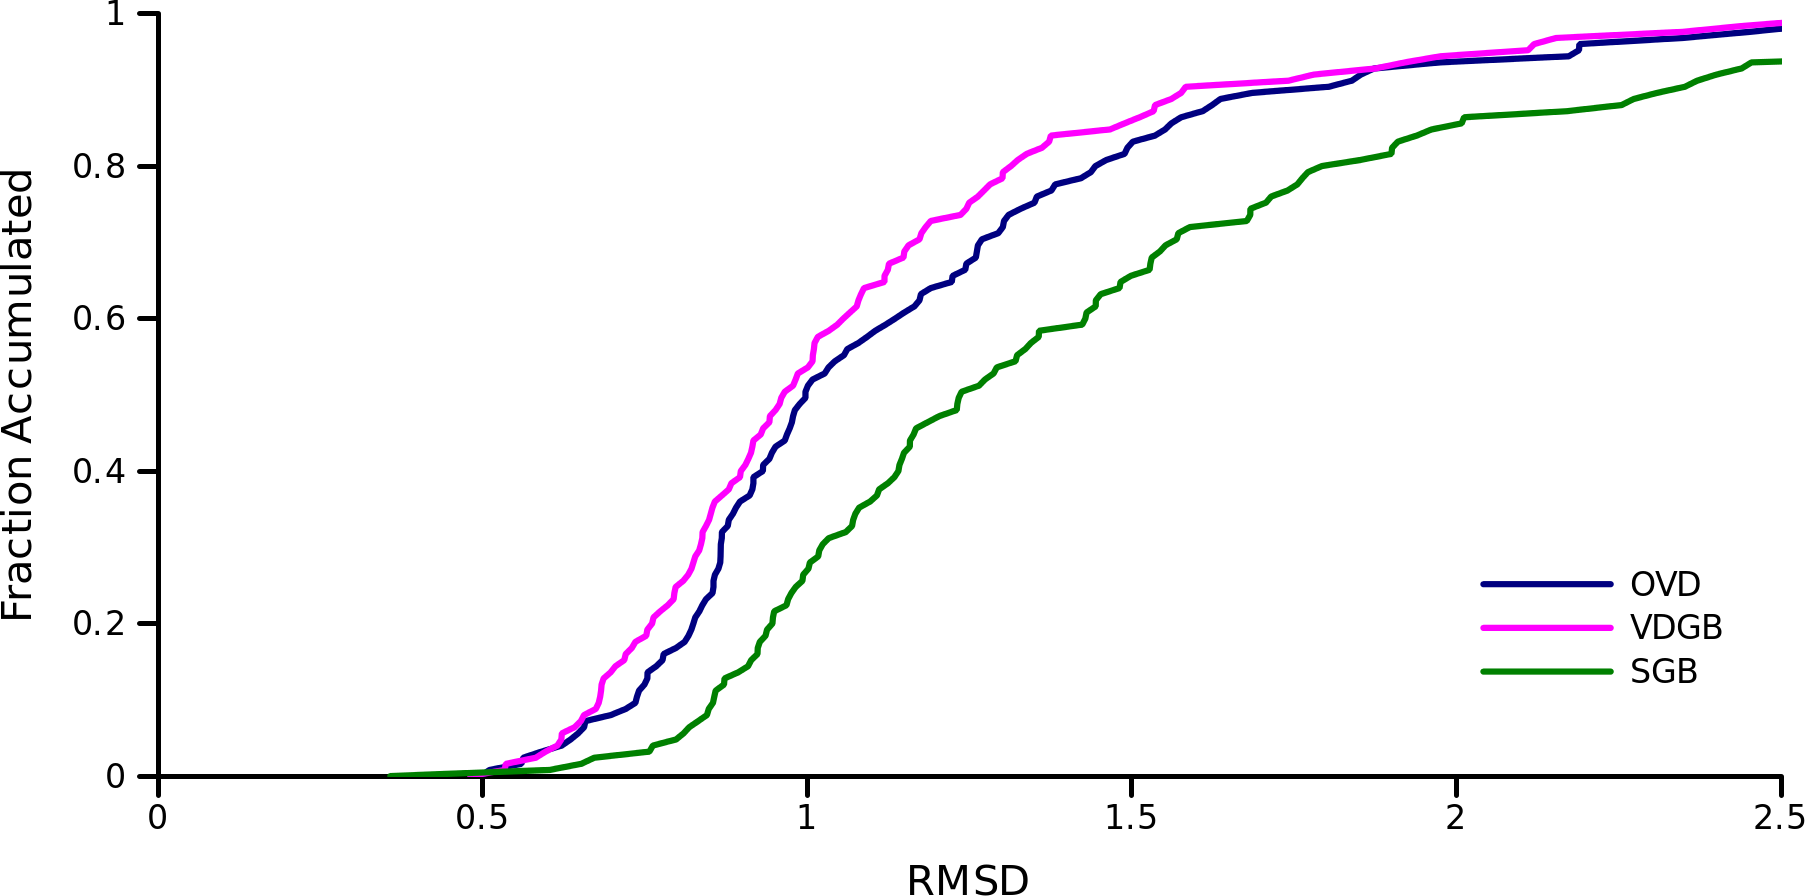
\includegraphics[width=0.8\textwidth]{figures/small_molecule_minimization.png}
\caption{The fraction of minimized structures found within a given RMSD to native.
The newer energy models, optimized variable dielectric (OVD or VSGB2.0) and variable dielectric surface generalized Born (VSGB) perform better than the original surface generalized Born model, however there is not significant differentiation between the two.}
\label{figure:small_molecule_minimization}
\end{figure}

The performance of a selection of the energy models implemented in PLOP was compared using a subset of these ligands found in CDK2 crystal structures.
Minimized crystal structures starting from the crystal coordinates were consistently closer to native conformations using the variable dielectric generalized Born solvation model than using a constant internal dielectric.
However, there was no differentiation found between the newer and significantly more complex energy model, variously named optimized variable dielectric (OVD) and variable dielectric surface generalized Born 2.0 (VSGB2.0) \cite{li2011vsgb}, which implements a number of terms to explicitly describe hydrogen bonding, $\pi-\pi$ interactions, and a number of other organic interactions.

In addition to adding support for a large number of small molecule ligands, a number of problems that plagued PDB loading have been corrected.
These included lacking support for a number of crystal symmetry groups, and erroneously loading modified amino acids as non-covalently bonded zwitterions.
This latter problem frequently led to steric clashes, as the free amino acid would clash with the free ends of the protein chain to which it should have been covalently bonded.
The energy involved in this sort of interaction is so severe that it would ``drown out'' small changes elsewhere in the system, though occasionally this could be worked around by freezing the coordinates of the problematic part of the protein structure.
